% Options for packages loaded elsewhere
\PassOptionsToPackage{unicode}{hyperref}
\PassOptionsToPackage{hyphens}{url}
%
\documentclass[
  a4paper, xcolor = usenames,dvipsnames]{article}
\usepackage{lmodern}
\usepackage{amssymb,amsmath}
\usepackage{ifxetex,ifluatex}
\ifnum 0\ifxetex 1\fi\ifluatex 1\fi=0 % if pdftex
  \usepackage[T1]{fontenc}
  \usepackage[utf8]{inputenc}
  \usepackage{textcomp} % provide euro and other symbols
\else % if luatex or xetex
  \usepackage{unicode-math}
  \defaultfontfeatures{Scale=MatchLowercase}
  \defaultfontfeatures[\rmfamily]{Ligatures=TeX,Scale=1}
\fi
% Use upquote if available, for straight quotes in verbatim environments
\IfFileExists{upquote.sty}{\usepackage{upquote}}{}
\IfFileExists{microtype.sty}{% use microtype if available
  \usepackage[]{microtype}
  \UseMicrotypeSet[protrusion]{basicmath} % disable protrusion for tt fonts
}{}
\makeatletter
\@ifundefined{KOMAClassName}{% if non-KOMA class
  \IfFileExists{parskip.sty}{%
    \usepackage{parskip}
  }{% else
    \setlength{\parindent}{0pt}
    \setlength{\parskip}{6pt plus 2pt minus 1pt}}
}{% if KOMA class
  \KOMAoptions{parskip=half}}
\makeatother
\usepackage{xcolor}
\IfFileExists{xurl.sty}{\usepackage{xurl}}{} % add URL line breaks if available
\IfFileExists{bookmark.sty}{\usepackage{bookmark}}{\usepackage{hyperref}}
\hypersetup{
  hidelinks,
  pdfcreator={LaTeX via pandoc}}
\urlstyle{same} % disable monospaced font for URLs
\usepackage[margin=2.5cm]{geometry}
\usepackage{listings}
\newcommand{\passthrough}[1]{#1}
\lstset{defaultdialect=[5.3]Lua}
\lstset{defaultdialect=[x86masm]Assembler}
\usepackage{longtable,booktabs}
% Correct order of tables after \paragraph or \subparagraph
\usepackage{etoolbox}
\makeatletter
\patchcmd\longtable{\par}{\if@noskipsec\mbox{}\fi\par}{}{}
\makeatother
% Allow footnotes in longtable head/foot
\IfFileExists{footnotehyper.sty}{\usepackage{footnotehyper}}{\usepackage{footnote}}
\makesavenoteenv{longtable}
\usepackage{graphicx}
\makeatletter
\def\maxwidth{\ifdim\Gin@nat@width>\linewidth\linewidth\else\Gin@nat@width\fi}
\def\maxheight{\ifdim\Gin@nat@height>\textheight\textheight\else\Gin@nat@height\fi}
\makeatother
% Scale images if necessary, so that they will not overflow the page
% margins by default, and it is still possible to overwrite the defaults
% using explicit options in \includegraphics[width, height, ...]{}
\setkeys{Gin}{width=\maxwidth,height=\maxheight,keepaspectratio}
% Set default figure placement to htbp
\makeatletter
\def\fps@figure{htbp}
\makeatother
\setlength{\emergencystretch}{3em} % prevent overfull lines
\providecommand{\tightlist}{%
  \setlength{\itemsep}{0pt}\setlength{\parskip}{0pt}}
\setcounter{secnumdepth}{5}
\usepackage{setspace}
\usepackage{float}
\usepackage{fontspec}
\usepackage{subfig}
\usepackage{hyperref}
\usepackage{multirow}
\usepackage{tikz}
\usetikzlibrary{chains,shapes.multipart}
\usetikzlibrary{shapes,calc,fit}
\usetikzlibrary{automata,positioning}
\floatplacement{figure}{H}
\makeatletter
\renewcommand\paragraph{\@startsection{paragraph}{4}{\z@}%
  {-2.5ex\@plus -1ex \@minus -.25ex}%
  {1.25ex \@plus .25ex}%
  {\normalfont\normalsize\bfseries}}
\makeatother
\setcounter{secnumdepth}{4}
\hypersetup{
  colorlinks = true,
}
\tikzset{
queuei/.pic={
  \draw[line width=1pt]
    (0,0) -- ++(2cm,0) -- ++(0,-1cm) -- ++(-2cm,0);
   \foreach \Val in {1,...,3}
     \draw ([xshift=-\Val*10pt]2cm,0) -- ++(0,-1cm);
   \node[above] at (1cm,0) {$c_{#1, m_{#1}}$};
   \node[] at (0.5cm,-0.5cm) (q-#1) {};   
  },
mytri/.style={
  draw,
  shape=isosceles triangle,
  isosceles triangle apex angle=60,
  inner xsep=0.65cm
  }
}

\author{}
\date{\vspace{-2.5em}}

\begin{document}

\onehalfspacing

\pagenumbering{gobble}

\vspace*{\fill}
\begin{center}
  \Large{\textbf{Internship report}}\\
  \vspace*{1\baselineskip}
  \Large{\textbf{Members}}\\
  Vo Van Nghia\\
  \vfill
  \vspace*{\fill}
  \Large{\textbf{Date}}\\
  29 Sep, 2022
\end{center}

\newpage

\newpage
\pagenumbering{roman}
\tableofcontents
\addcontentsline{toc}{section}{\contentsname}

\newpage
\pagenumbering{arabic}

\hypertarget{introduction}{%
\section{Introduction}\label{introduction}}

\hypertarget{institut-de-recherche-en-informatique-de-toulouse-irit}{%
\subsection{Institut de Recherche en Informatique de Toulouse (IRIT)}\label{institut-de-recherche-en-informatique-de-toulouse-irit}}

\hypertarget{about-the-institut}{%
\subsubsection{About the institut}\label{about-the-institut}}

The Institut de Recherche en Informatique de Toulouse (IRIT), created in 1990, is a Joint Research Unit (UMR 5505) of the Centre National de la Recherche Scientifique (CNRS), the Institut National Polytechnique de Toulouse (INP), the Université Paul Sabatier Toulouse3 (UT3), the Université Toulouse1 Capitole (UT1) and the Université de Toulouse Jean Jaurès (UT2J).

IRIT is one of the largest UMR at the national level, is one of the pillars of research in Occitanie with its 600 members, permanent and non-permanent, and about 100 external collaborators. Due to its multi-tutorial nature (CNRS, Toulouse Universities), its scientific impact and its interactions with other fields, the laboratory constitutes one of the structuring forces of the IT landscape and its applications in the digital world, both at regional and national level.

Through its cutting-edge work and dynamics, our unit has been able to define its identity and acquire undeniable visibility, while positioning itself at the heart of changes in local structures: University of Toulouse, as well as the various mechanisms resulting from future investments (LabEx CIMI, IRT Saint-Exupéry, SAT TTT, 3IA ANITI).

IRIT has focused its research on five major scientific issues and six strategic application areas.

\begin{itemize}
\tightlist
\item
  Health, Autonomy, Living, Well-being
\item
  Smart City
\item
  Aerospace and Transportation
\item
  Social Media, Digital Social Ecosystems
\item
  e-Education for learning and teaching
\item
  Heritage and People Safety
\end{itemize}

As well as strategic action:

\begin{itemize}
\tightlist
\item
  Scientific Computing, Big Data and AI
\end{itemize}

\hypertarget{organization}{%
\subsubsection{Organization}\label{organization}}

The 24 research groups of the laboratory are dispatched in seven scientific departments:

\begin{itemize}
\tightlist
\item
  Dpt ASR : Architecture, Systems, Networks
\item
  Dpt CISO : HPC, Simulation, Optimization
\item
  Dpt FSL : Reliability of Systems and Software
\item
  Dpt GD : Data Management
\item
  Dpt ICI : Interaction, Collective Intelligence
\item
  Dpt IA : Artificial Intelligence
\item
  Dpt SI : Signals, Images
\end{itemize}

\hypertarget{the-internship}{%
\subsection{The internship}\label{the-internship}}

Markov decisions processes (MDPs) and their model free counterpart in reinforcement learning (RL) have known a large success in the last two decades. Although research in these two areas has been taking place for more than fifty years, the field gained momentum only recently following the advent of powerful hardware and algorithms with which supra­human performance were obtained in games like Chess or Go. However, these impressive successes often rely on quite exceptional hardware possibilities and cannot be applied in many ''usual'' contexts, where, for instance, the volume of data available or the amount of computing power is more restricted. To define the next generation of more ''democratic'' and widely applicable algorithms, such methods still need to deal with very demanding exploration issues as soon as the state/action spaces are not small. One way around this is to use underlying knowledge and structure present in many MDPs. This is especially true for problems related to scheduling and resources sharing in among others server farms, clouds, and cellular wireless networks. The internships will revolve around this theme of improving the efficiency of learning algorithms by leveraging the structure of the underlying problem and focus mainly on model­free approach.

\hypertarget{problem-settings}{%
\section{Problem settings}\label{problem-settings}}

Two type of systems are studied in this internship: queuing system and load-balancing system.

\hypertarget{queuing-system}{%
\subsection{Queuing system}\label{queuing-system}}

\hypertarget{describe}{%
\subsubsection{Describe}\label{describe}}

We have \(n\) classes of queue \(C_{1}, \dots, C_{n}\). For each class of queue, its behavior is fully controlled by which environment it is in. An environment can be in one of the states \(m_{1}, \dots, m_{m}\). And the environment of class \(C_{i}\) is a random variable, denoted by \(M_{i}\), which is in one of the states \(m_{1}, \dots, m_{m}\). For each environment, \(C_{i}\) has their own holding cost \(c_{i, j}\) (the cost of one unfinished unit of work on the queue), arrival rate \(\lambda_{i, j}\) (the rate of one more unit of work arriving to the queue) and departure rate \(\mu_{i, j}\) (the rate of one unit of work on the queue has finished). Furthermore, the environment \(M_{i}\) can change from \(m_{j}\) and \(m_{k}\) with the rate of \(\xi_{i, j, k}\). A table summarizing all parameters is shown below.

\begin{table}[ht]
\caption{Queuing system parameters}
\begin{center}
\begin{tabular}{c c c c c}
    \hline
    \multicolumn{2}{c}{} & $m_{1}$ & $\dots$ & $m_{m}$ \\
    \cline{2-5}
    \multirow{3}{*}{$C_{1}$} &  Holding cost & $c_{1, 1}$ & $\dots$ & $c_{1, m}$ \\
    & Arrival rate & $\lambda_{1, 1}$ & $\dots$ & $\lambda_{1, m}$ \\
    & Departure rate & $\mu_{1, 1}$ & $\dots$ & $\mu_{1, m}$ \\
    \cline{2-5}
    $\vdots$  \\
    \cline{2-5}
    \multirow{3}{*}{$C_{n}$} &  Holding cost & $c_{n, 1}$ & $\dots$ & $c_{n, m}$ \\
    & Arrival rate & $\lambda_{n, 1}$ & $\dots$ & $\lambda_{n, m}$ \\
    & Departure rate & $\mu_{n, 1}$ & $\dots$ & $\mu_{n, m}$ \\
    \hline
\end{tabular}
\end{center}
\label{tab:qs-param}
\end{table}

For each \(C_{i}\), we have a matrix transition as below.

\begin{table}[ht]
\caption{Matrix transition of the environment of $C_{i}$}
\begin{center}
\begin{tabular}{c c c c}
    \hline
    & $m_{1}$ & $\dots$ & $m_{m}$ \\
    $m_{1}$ & $\xi_{i, 1, 1}$ & \dots & $\xi_{i, 1, m}$ \\
    \vdots \\
    $m_{m}$ & $\xi_{i, m, 1}$ & \dots & $\xi_{i, m, m}$ \\
    \hline
\end{tabular}
\end{center}
\label{tab:mat-transition-ci}
\end{table}

The agent will decide which queues should be activated. Only works on activating queues can be processed and finished. In more generic problems, the agent is allowed to activate / deactivate multiple queues at the same time based on some conditions. However, in this internship, the agent can only activate one queue at a time.

\begin{figure}
\centering
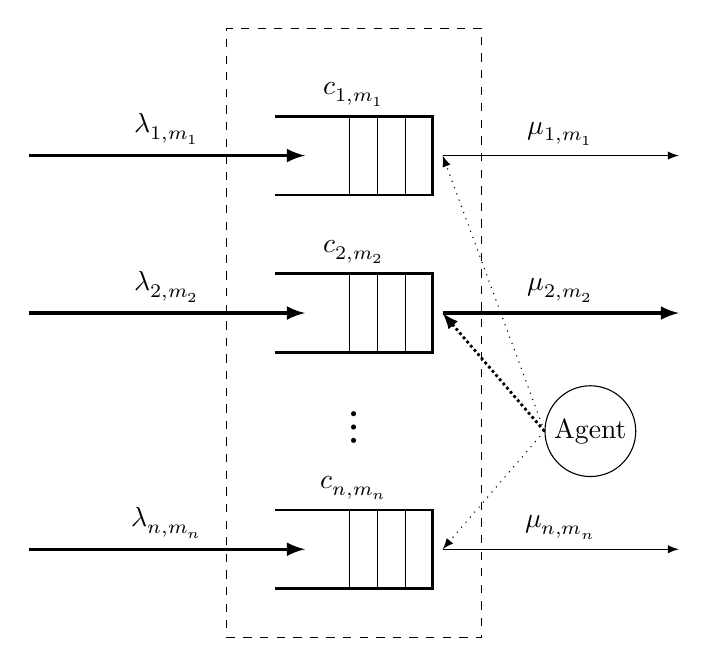
\begin{tikzpicture}[>=latex]
% the shapes
\path
  (0,3cm) pic {queuei=1}
  (0,1cm) pic {queuei=2}
  (0,-2cm) pic {queuei=n};
\path
  (1,4cm) coordinate (aux1)
  (1,-3.5cm) coordinate (aux2)
  (-0.5,0cm) coordinate (aux3)
  (2.5,0cm) coordinate (aux4);
\node[draw,dashed,text width=2.5cm,fit={(aux1) (aux2) (aux3) (aux4)}] (dashed) {};
\node[draw,align=center,circle,inner sep=2pt]
  at (4,-1) (agent)
  {Agent};

%the arrows
\draw[->, line width=1.25]
  ([xshift=-3.5cm]q-1.west) --
    node[anchor=south,align=center] {$\lambda_{1, m_{1}}$}
  (q-1.west);
\draw[->]
  ([xshift=1.5cm]q-1.east) --
    node[anchor=south,align=center] {$\mu_{1, m_{1}}$}
  ([xshift=4.5cm]q-1.east);
\draw[->, line width=1.25]
  ([xshift=-3.5cm]q-2.west) --
    node[anchor=south,align=center] {$\lambda_{2, m_{2}}$}
  (q-2.west);
\draw[->, line width=1.25]
  ([xshift=1.5cm]q-2.east) --
    node[anchor=south,align=center] {$\mu_{2, m_{2}}$}
  ([xshift=4.5cm]q-2.east);
\draw[->, line width=1.25]
  ([xshift=-3.5cm]q-n.west) --
    node[anchor=south,align=center] {$\lambda_{n, m_{n}}$}
  (q-n.west);
\draw[->]
  ([xshift=1.5cm]q-n.east) --
    node[anchor=south,align=center] {$\mu_{n, m_{n}}$}
  ([xshift=4.5cm]q-n.east);
\draw[->,dotted]
  (agent.west) --
    node[anchor=south,align=center] {}
  ([xshift=1.5cm]q-1.east);
\draw[->,densely dotted, line width=1]
  (agent.west) --
    node[anchor=south,align=center] {}
  ([xshift=1.5cm]q-2.east);
\draw[->,dotted]
  (agent.west) --
    node[anchor=south,align=center] {}
  ([xshift=1.5cm]q-n.east);
\path ([xshift=0.5cm]q-2.south) -- ([xshift=0.5cm]q-n.north) node [font=\LARGE, midway, sloped] {$\dots$};
\end{tikzpicture}
\caption[Visualization of the queueing system when the agent activates queue 2]{Visualization of the queueing system when the agent activates queue 2, the bold lines represent the flow of works inside the system.}
\end{figure}

The state of the system is represented by two vectors:

\begin{itemize}
\tightlist
\item
  \(S = (X_{1}, \dots, X_{n})\) where \(X_{i}\) is a random variable represents the current number of works of class \(C_{i}\) and is observable.
\item
  \(E = (M_{1}, \dots, M_{n})\) and this vector is not observable.
\end{itemize}

\end{document}
